\documentclass[tikz, border=10pt]{standalone}
\usepackage{pgfplots}
\usepackage{siunitx}
\pgfplotsset{compat=1.18}

\begin{document}
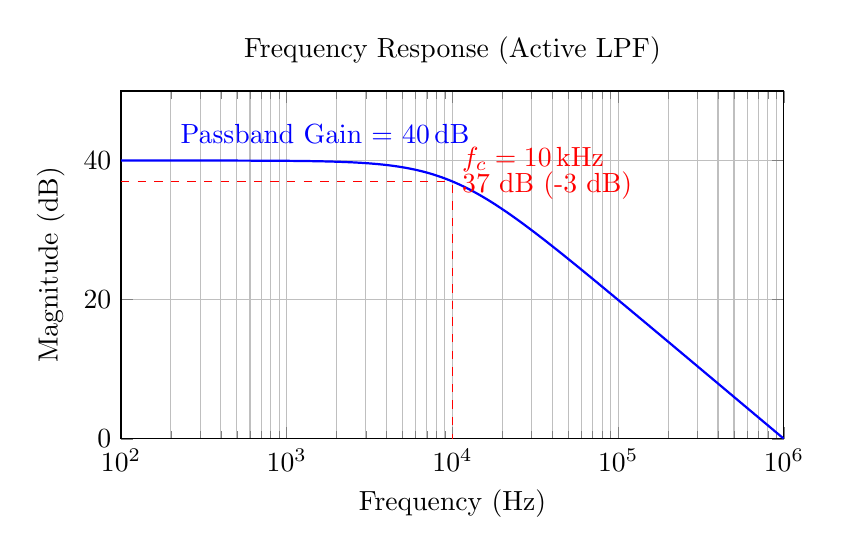
\begin{tikzpicture}
    \begin{semilogxaxis}[
        width=10cm, height=6cm,
        title={Frequency Response (Active LPF)},
        xlabel={Frequency (Hz)},
        ylabel={Magnitude (dB)},
        grid=both,
        xmin=100, xmax=1e6,
        ymin=0, ymax=50,
        samples=500,
        domain=100:1e6,
    ]
    
    % Parameters
    % K = 100 (40 dB)
    % fc = 10 kHz = 1e4
    % H(f) = K / sqrt(1 + (f/fc)^2)
    % |H| dB = 20 log10( |H| )
    
    \addplot[thick, blue, variable=\f] 
    { 20 * log10( 100 / sqrt(1 + (\f/1e4)^2) ) };
    
    % Mark Cutoff
    \draw[dashed, red] (axis cs: 1e4, -10) -- (axis cs: 1e4, 37);
    \draw[dashed, red] (axis cs: 100, 37) -- (axis cs: 1e4, 37);
    
    \node[anchor=south west, red] at (axis cs: 1e4, 37) {$f_c = \SI{10}{kHz}$};
    \node[anchor=south west, red] at (axis cs: 1e4, 33) {37 dB (-3 dB)};
    \node[anchor=south west, blue] at (axis cs: 200, 41) {Passband Gain = \SI{40}{dB}};
    
    \end{semilogxaxis}
\end{tikzpicture}
\end{document}
